%! Author = joaopintosp
%! Date = 8/25/24
\section{Introdução}\label{sec:introducao}

    The \ac{t} was measured using a thermometer.
    Also, it was verified that the \ac{t} was extremely hot.


    \lipsum[1]

    \subsection{Motivo}\label{subsec:motivo}

    Isto é apenas uma introdução para ver se gosto ou não de utilizar o Pycharm com \LaTeX.
    Pode ser que se torne a minha nova ferramenta de trabalho, sendo que em 2025 começarei a minha dissertação de mestrado.
    \lipsum[1]

    \subsection{Ortografia}\label{subsec:ortografia}

    Será que o Pycharm corrige a ortografia?
    Pelos vistos, sim!
    O Pycharm corrige a ortografia.
    \lipsum[2]

    \paragraph{Parágrafo da Introdução} \lipsum[3]

    \subsection{Figuras e Tabelas}\label{subsec:figuras-e-tabelas}

    Aqui está uma tabela:

    \begin{table}[htb!]
        \centering
        \begin{tabular}{lrr}
\toprule
name & age & height \\
\midrule
FREDERICO & 24 & 170.8 \\
DONATELLO & 45 & 177.7 \\
\bottomrule
\end{tabular}

        \caption{Uma tabela.}\label{tab:tabela}
    \end{table}

    Write some text.
    Como mostrado na Tabela~\ref{tab:tabela}. \lipsum[5]

    Aqui está uma figura.
    Esta é a Figura~\ref{fig:figure}:
    \begin{figure}[htb!]
        \centering
        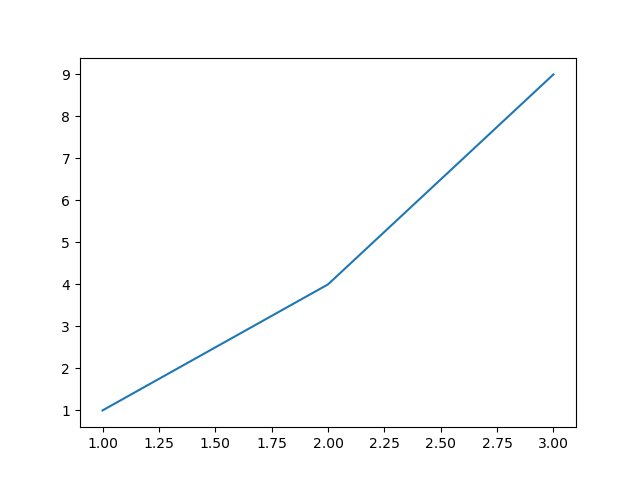
\includegraphics[width=0.5\textwidth]{figures/figure}
        \caption{Isto é um plot.}\label{fig:figure}
    \end{figure}

    \newpage

    Aqui está uma subfigura:

    \begin{figure}[htb!]
        \centering
        \begin{subfigure}[b]{0.45\textwidth}
             \centering
             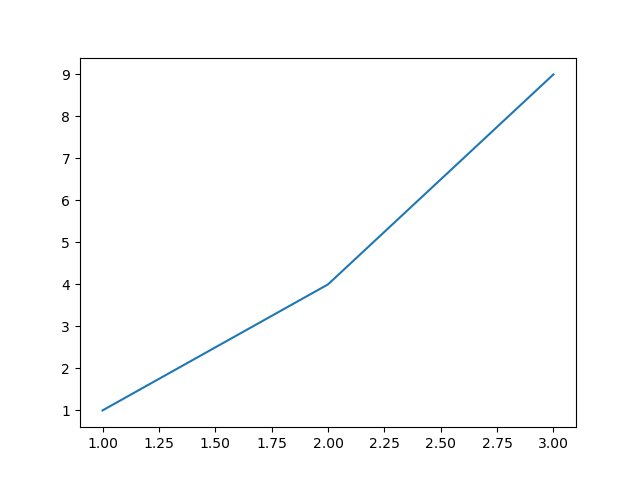
\includegraphics[width=\textwidth]{figures/figure}
             \caption{$y=3\sin x$}
             \label{fig:three sin x}
         \end{subfigure}
         \hfill
         \begin{subfigure}[b]{0.45\textwidth}
             \centering
             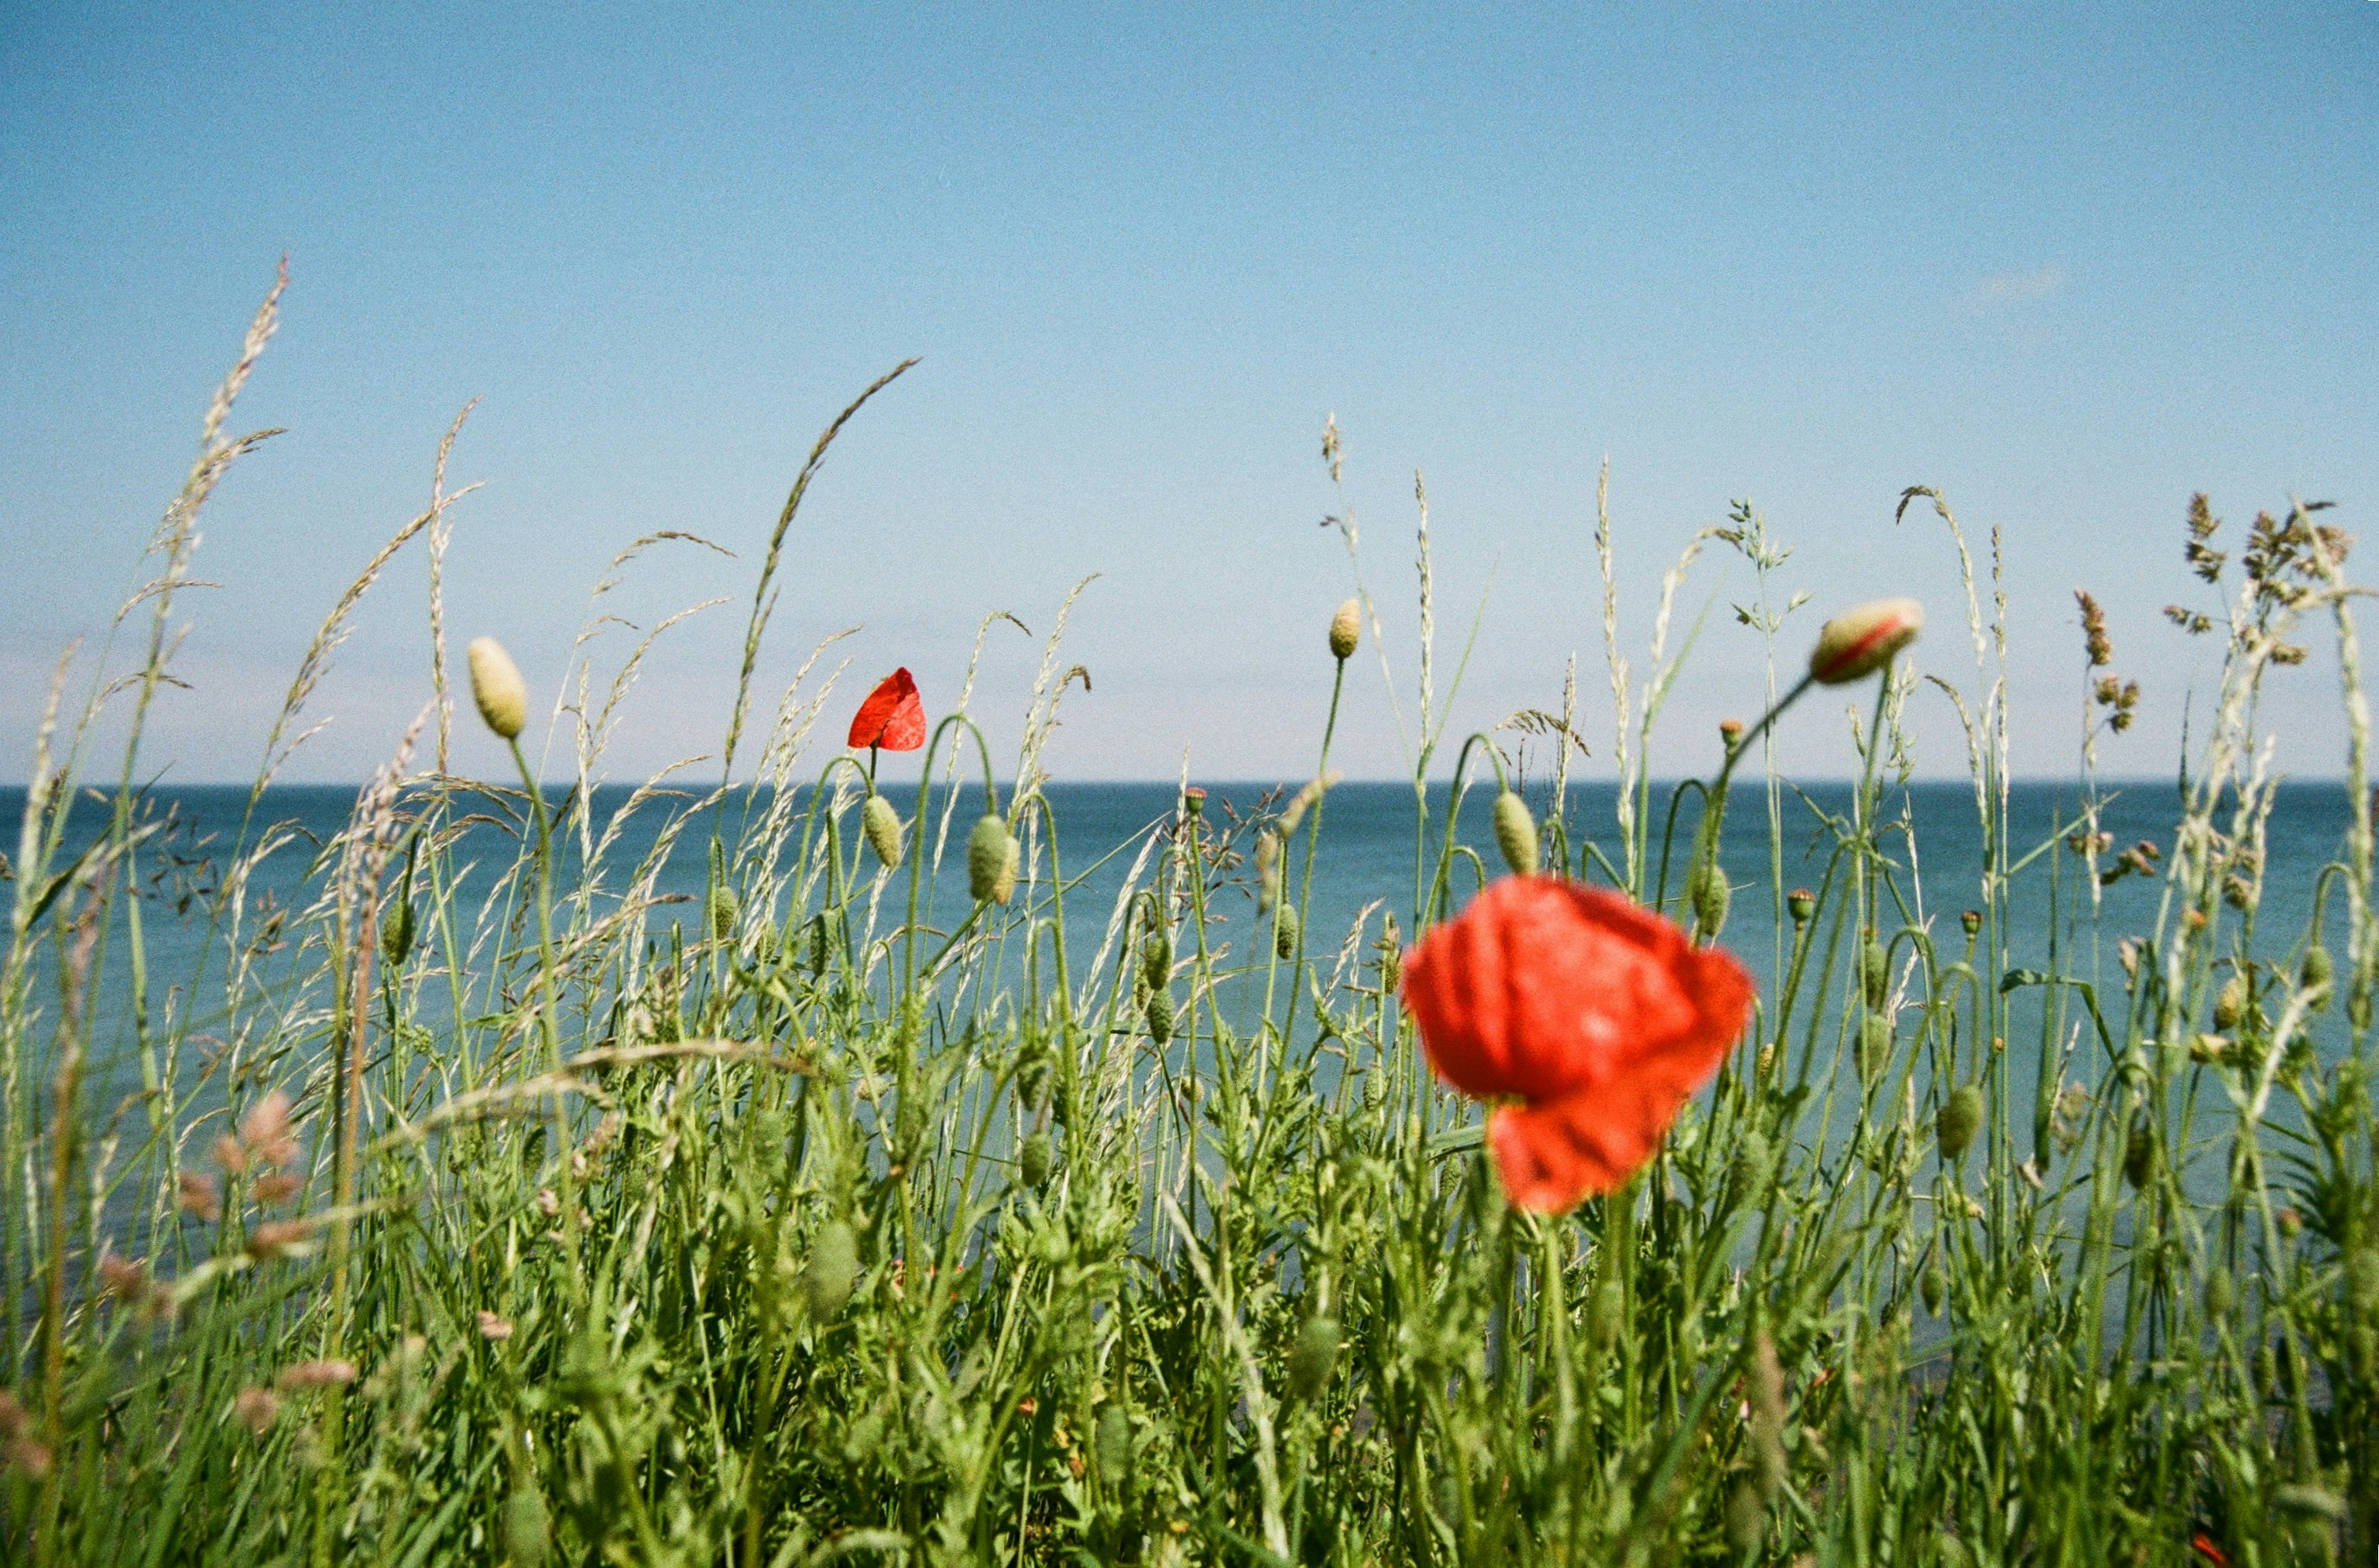
\includegraphics[width=\textwidth]{figures/flores}
             \caption{$y=5/x$}
             \label{fig:five over x}
         \end{subfigure}
            \caption{Duas simples figuras.}
            \label{fig:twographs}
    \end{figure}

    A Figura~\ref{fig:twographs} é composta por duas subfiguras, a Figura~\ref{fig:three sin x} e a Figura~\ref{fig:five over x}.